\chapter{Opis projektnog zadatka}
		
		Cilj ovog projekta je razviti programsku podršku za stvaranje web aplikacije „Iznajmi romobil“ koja će korisnicima omogućiti da iznajme svoj električni romobil u periodima dana kada ga ne koriste. Pomoću aplikacije korisnici će moći brzo i jednostavno pristupiti električnim romobilima dostupnima za najam kao i postaviti ponudu za iznajmljivanje svog romobila. Električni romobili danas su odlična alternativa za automobile te zbog svoje ekološke prihvatljivosti i praktičnosti postaju sve popularniji u većim urbanim sredinama. Korisnik koji želi iznajmiti svoj romobil, prilikom registracije romobila, unosi osnovne informacije o romobilu. Kada je romobil registriran, za njega se može objaviti oglas za iznajmljivanje pri čemu vlasnik upisuje gdje se romobil trenutno nalazi te gdje i kada mora biti vraćen. Korisnik koji želi unajmiti romobil, na temelju ponuđenih romobila i informacija o njima odabire onaj koji je u tom trenutku dostupan i najviše odgovara njegovim potrebama. 
		\newline 
		\newline
		Prilikom pokretanja aplikacije, korisnicima se neovisno o tome jesu li prijavljeni ili ne prikazuje popis svih aktivnih oglasa romobila. Uz svaki su romobil navedene njegove karakteristike, cijena, lokacija na kojoj se romobil nalazi te vrijeme i lokacija gdje romobil mora biti vraćen. \textbf{Neregistrirani korisnici} mogu pregledavati trenutno dostupne romobile i njihova cijene, ali ih ne mogu iznajmiti. Nakon što kreiraju novi korisnički račun, ponuđeni romobili im postaju dostupni za najam. Prilikom kreiranja novog računa korisnici moraju unijeti sljedeće podatke:
		
		\begin{packed_item}
			\item \textit{ime i prezime}
			\item \textit{email adresa}
			\item \textit{nadimak}
			\item \textit{broj kartice}
		\end{packed_item}
		
		Osim navedenog, korisnici prilikom registracije moraju dostaviti kopiju osobne iskaznice i potvrdu o nekažnjavanju. Nakon što su uneseni svi podaci i dostavljeni potrebni dokumenti, korisnik čeka pregled dokumenata odnosno odobravanje ili odbijanje registracije. Dok registracija nije odobrena, korisnik se ne može prijaviti u sustav. Ako je zahtjev za registraciju odbijen zbog neispravnosti dostavljenih dokumenata, korisnik može ponovno predati dokumente. Korisnici koji su unaprijed registrirani, mogu se prijaviti u sustav sa svojim postojećim korisničkim računom tako da unesu email adresu i lozinku. Ako korisnik prilikom unosa podataka za prijavu unese podatke koji ne odgovaraju nijednom registriranom korisniku u bazi, šalje mu se obavijest o neispravnosti podataka. \textbf{Klijent} je korisnik aplikacije koji može pregledavati i unajmljivati romobile, ali nema registriranih vlastitih romobila. Kada odabere romobil koji želi unajmiti, klijent se javlja na oglas s automatski generiranom porukom koja sadrži zahtjev za unajmljivanje. Nakon što je ponuda prihvaćena, klijentu se šalje obavijest da je iznajmljivanje odobreno i oglas se briše. Klijent prije pokretanja romobila provjerava odgovara li fotografija romobila njegovom stvarnom stanju. Ako ne odgovara, on ima mogućnost odabirom opcije "Zamijeni sliku" zamijeniti sliku romobila novom slikom i kratkim opisom o razlikama između nove i stare slike. Na kraju iznajmljivanja, klijent vraća romobil i u aplikaciji potvrđuje da ga je vratio. Nakon toga slijedi provjera je li romobil vraćen u pravo vrijeme te se izračunava cijena koju klijent mora platiti. Svaki klijent u aplikaciji može pregledati svoj profil na kojem se nalaze njegovi osobni podaci. Za sve podatke on sam određuje hoće li oni biti javno dostupni ili ne, a iste može urediti odabirom opcije "Uredi profil".  Pri uređivanju profila provjerava se jesu li novi podatci uneseni u ispravnom formatu, ako nisu korisnik dobiva obavijest o neispravnosti. Nakon unosa promjena, klijent mora odabrati opciju "Spremi promjene" kako bi potvrdio pohranjivanje promjena u bazu podataka. Na profilu svakog klijenta moraju biti vidljive ocjene i komentari iznajmljivača. Klijent, u trenutku kada registrira svoj romobil, postaje \textbf{iznajmljivač}. Prilikom registracije romobila potrebno je unijeti sljedeće podatke o romobilu: 
		
			\begin{packed_item}
			\item \textit{naziv proizvođača}
			\item \textit{naziv modela}
			\item \textit{kapacitet baterije}
			\item \textit{maksimalna brzina}
			\item \textit{URL fotografije romobila}
			\item \textit{maksimalni domet}
			\item \textit{godina proizvodnje}
			\item \textit{dostupnost}
			\item \textit{dodatne informacije (po želji)}
			\end{packed_item}
			
		Prilikom postavljanja ponude za iznajmljivanje, iznajmljivač unosi trenutnu lokaciju romobila, lokaciju na koju želi da se romobil vrati, vrijeme do kada romobil mora biti vraćen, cijenu iznajmljivanja po prijeđenom kilometru te iznos novčane kazne u slučaju da romobil ne bude vraćen na vrijeme. Ako je neki romobil dostupan za iznajmljivanje, iznajmljivač oglas može podijeliti i na nekoj društvenoj mreži odabirom opcije "Objavi na društvenu mrežu". Svaki iznajmljivač može pregledavati svoje registrirane romobile, brisati postojeće i dodavati nove. Ako iznajmljivač izbriše sve svoje registrirane romobile, ono ponovno postaje klijent. Unutar aplikacije dostupna je mogućnost izmjenjivanja poruka kako bi se klijent i iznajmljivač mogli dogovoriti oko najma. Iznajmljivač pregledava zahtjeve za iznajmljivanje i profile klijenata te tada može prihvatiti ili odbiti ponudu. Ako klijent zamijeni sliku romobila jer smatra da ne prikazuje stvarno stanje romobila, iznajmljivaču se šalje obavijest o zamjeni. On tada, ako smatra da klijentova slika nije ispravna, može poslati žalbu na zamjenu slika. Nakon što administrator donese odluku o zamjeni slika, klijentu i iznajmljivaču se šalje obavijest o donesenoj odluci. Na kraju iznajmljivanja, iznajmljivač kao i klijent dobiva obavijest da je iznajmljivanje završeno i cijenu iznajmljivanja koju mu klijent treba platiti. Iznajmljivač nakon završetka iznajmljivanja može ocijeniti klijenta i napisati komentar. \textbf{Administrator} pregledava dokumente dostavljene prilikom registracije, odbija ili prihvaća zahtjeve za registraciju, dodjeljuje nove uloge administratora te iste briše. Osim toga, on zaprima žalbe na zamjenu slika romobila. Nakon zaprimanja žalbe administrator pregledava slike i odabire onu koja će se pohraniti u bazu. Administrator ima pravo blokirati korisnika odnosno zabraniti mu pristup aplikaciji odabirom opcije "Blokiraj korisnika". Za takvog se korisnika u bazu podataka upisuje da je blokiran te će mu pri sljedećoj prijavi biti onemogućen pristup sustavu.
		\newline
		\newline
		Ovaj način izvedbe aplikacije bi definitivno bio koristan za današnje društvo. Kori- štenje aplikacije pridonijelo bi smanjenju emisija štetnih plinova i gužve te poveća- nju mobilnosti. Električni romobili, kao što im naziv govori pokreću se električnom energijom te kao takvi doprinose smanjenju emisija štetnih plinova i zagađenja zraka. Kada bi se povećao broj korisnika električnih romobila odnosno kada bi ljudi umjesto automobila i taksija koristili električne romobile, smanjili bi se prometni zastoji te bi se poboljšala fluidnost prometa. Široka rasprostranjenost romobila po gradu i jednostavno pronalaženje oglasa povećali bi dostupnost prijevoza. Osim navedenih prednosti, aplikacija bi iznajmljivačima omogućila dodatni prihod od iznajmljivanja romobila u periodima kada ga ne koriste, čime se maksimizira iskorištavanje resursa i potiče održiv način dijeljenja prijevoznih sredstava. Aplikacija je namijenjena stanovnicima urbanih sredina i turistima, pružajući praktično rješenje za brz i ekološki prihvatljiv prijevoz. Stanovnici gradova mogu iskoristiti romobile kao učinkovito sredstvo prijevoza između odredišta te mogu iznajmljivati svoje romobile, dok turisti mogu istraživati grad na jednostavan način, dodatno obogaćujući svoje iskustvo boravka. Aplikacija bi se mogla unaprijediti tako da web aplikaciju pretvorimo u mobilnu kako bi se olakšala njena upotreba i dodale dodatne funkcionalnosti koje bi ju učinile još popularnijom.  
		\newline
		\newline
		Danas, kako električni romobili postaju sve popularniji, susrećemo se s mnogo sličnih aplikacija koje su aktivne u svim većim gradovima u svijetu. Nažalost, u Hrvatskoj takve aplikacije i mogućnost najma i iznajmljivanja i dalje nisu dostupne u većini gradova. Ključna razlika između aplikacije Iznajmi romobil i postojećih rješenja jest ta što su sve izvedene u obliku mobilnih aplikacija te uglavnom vlasnik aplikacije iznajmljuje veći broj svojih romobila što znači da korisnici mogu unajmiti romobile na aplikaciji, ali ne i iznajmiti svoje. Ta je razlika upravo prednost aplikacije Iznajmi romobil jer svi korisnici mogu objaviti oglas za svoj romobil, neovisno o tome imaju li jedan romobil ili više njih. Primjer sličnog rješenja u obliku mobilne aplikacije jest Bird. Bird je mobilna aplikacija koja korisnicima omogućuje najam električnih romobila i bicikala. Romobili i bicikli se nalaze na više lokacija u gradovima. Korisnici se prilikom pokretanja aplikacije registriraju odnosno prijave u sustav, a nakon toga na mapi pronađu gdje se nalazi najbliži romobil/bicikl dostupan za najam. Kada dođu do te točke, odaberu romobil/bicikl, skeniraju QR kod na njemu i započinju svoju vožnju. Cijena najma ovisi o lokaciji, a računa se prema pređenim kilometrima. Po završetku vožnje, u aplikaciji se označava da je vožnja završena, romobil/bicikl se ostavlja na za to predviđenom mjestu, a cijena najma naplaćuje se s bankovnog računa povezanog na korisnikov profil. Neke od dodatnih mogućnosti koje aplikacija nudi su zakazivanja grupnih vožnji što je iznimno pogodno za turističke skupine, rezervacija vozila do 30 minuta unaprijed te brojne cjenovne pogodnosti za stalne korisnike.
		
	

		\begin{figure} [H]
			
			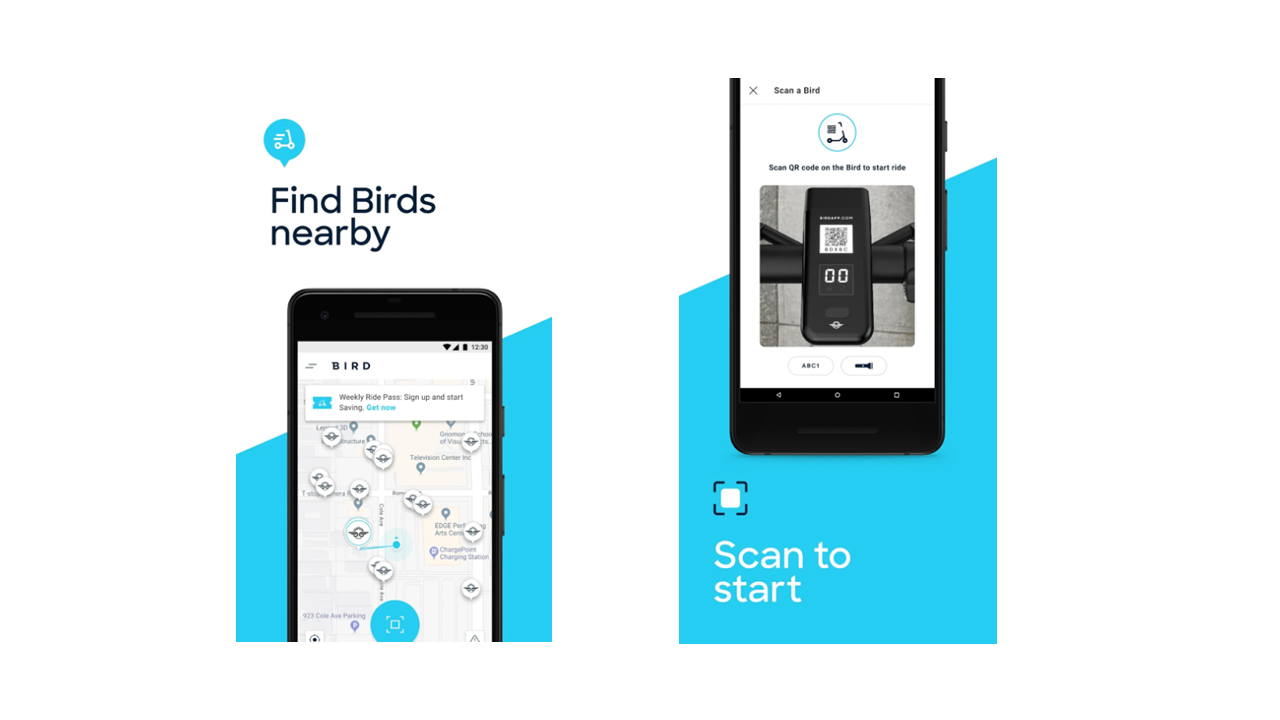
\includegraphics[width=1\linewidth]{slike/BirdApp1.png}
			\centering
			\caption{Prikaz pronalaska romobila i početka vožnje}
			\label{fig:Prikaz pronalaska romobila i započinjanja vožnje}
		\end{figure}
		
		\begin{figure} [H]
			
			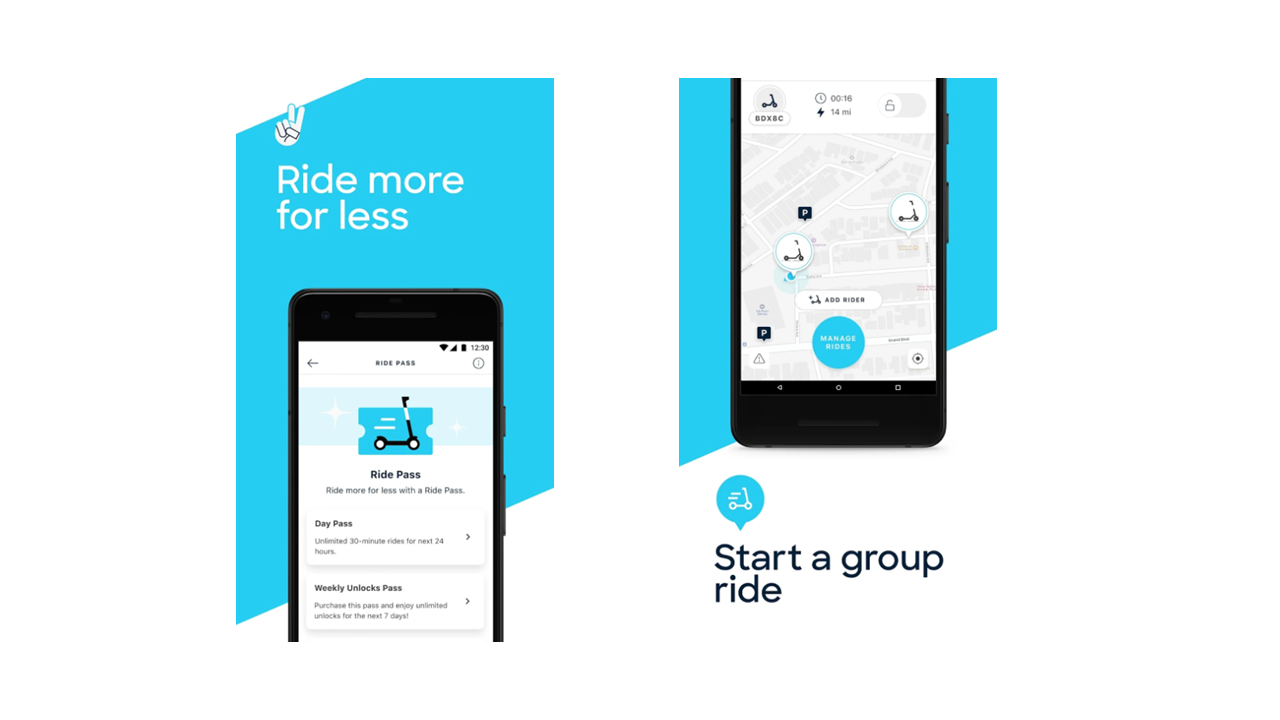
\includegraphics[width=1\linewidth]{slike/BirdApp2.png}
			\centering
			\caption{Prikaz dodatnih mogućnosti}
			\label{fig:Prikaz dodatnih mogućnosti}
		\end{figure}
		
		
		
		
		
		
		
	